
\documentclass[letterpaper,hide notes,xcolor={table,svgnames},pdftex,10pt]{beamer}
\def\showexamples{t}

\usecolortheme{crane}
\setbeamertemplate{navigation symbols}{}

\usetheme{MyPittsburgh}
\usepackage{hyperref}
\usepackage{graphicx,xspace}
\usepackage[normalem]{ulem}
\usepackage{multicol}
\usepackage{amsmath,amssymb,amsthm,graphicx,xspace}
\newcommand\SF[1]{$\bigstar$\footnote{SF: #1}}

\usepackage[sfdefault,lf]{carlito}
\usepackage[T1]{fontenc}
\usepackage[scaled]{beramono}
\usepackage{tikzpagenodes}
\newcommand{\Rplus}{\protect\hspace{-.1em}\protect\raisebox{.35ex}{\small{\small\textbf{+}}}}
\newcommand{\Cpp}{\mbox{C\Rplus\Rplus}\xspace}

\newcounter{tmpnumSlide}
\newcounter{tmpnumNote}

\newcommand\mnote[1]{%
	\addtocounter{tmpnumSlide}{1}
	\ifdefined\showcues {~\tiny\fbox{\arabic{tmpnumSlide}}}\fi
	\note{\setlength{\parskip}{1ex}\addtocounter{tmpnumNote}{1}\textbf{\Large \arabic{tmpnumNote}:} {#1\par}}}

\newcommand\mmnote[1]{\note{\setlength{\parskip}{1ex}#1\par}}


\newcommand\mquestion[2]{{~\color{red}\fbox{?}}\note{\setlength{\parskip}{1ex}\par{\Large \textbf{?}} #1} \note{\setlength{\parskip}{1ex}\par{\Large \textbf{A}} #2\par}\ifdefined \presentationonly \pause \fi}

\newcommand\blackboard[1]{%
	\ifdefined   \showblackboard
		{#1}
	\else {\begin{center} \fbox{\colorbox{blue!30}{%
						\begin{minipage}{.95\linewidth}%
							\hspace{\stretch{1}} Some space intentionally left blank; done at the blackboard.%
						\end{minipage}}}\end{center}}%
	\fi%
}

\usepackage{listings}
\lstset{%
	keywordstyle=\bfseries,
	aboveskip=15pt,
	belowskip=15pt,
	captionpos=b,
	identifierstyle=\ttfamily,
	frame=lines,
	numbers=left, basicstyle=\scriptsize, numberstyle=\tiny, stepnumber=0, numbersep=2pt}

\usepackage{siunitx}
\newcommand\sius[1]{\num[group-separator = {,}]{#1}\si{\micro\second}}
\newcommand\sims[1]{\num[group-separator = {,}]{#1}\si{\milli\second}}
\newcommand\sins[1]{\num[group-separator = {,}]{#1}\si{\nano\second}}
\sisetup{group-separator = {,}, group-digits = true}

%% -------------------- tikz --------------------
\usepackage{tikz}
\usetikzlibrary{positioning}
\usetikzlibrary{arrows,backgrounds,automata,decorations.shapes,decorations.pathmorphing,decorations.markings,decorations.text}

\tikzstyle{place}=[circle,draw=blue!50,fill=blue!20,thick, inner sep=0pt,minimum size=6mm]
\tikzstyle{transition}=[rectangle,draw=black!50,fill=black!20,thick, inner sep=0pt,minimum size=4mm]

\tikzstyle{block}=[rectangle,draw=black, thick, inner sep=5pt]
\tikzstyle{bullet}=[circle,draw=black, fill=black, thin, inner sep=2pt]

\tikzstyle{pre}=[<-,shorten <=1pt,>=stealth',semithick]
\tikzstyle{post}=[->,shorten >=1pt,>=stealth',semithick]
\tikzstyle{bi}=[<->,shorten >=1pt,shorten <=1pt, >=stealth',semithick]

\tikzstyle{mut}=[-,>=stealth',semithick]

\tikzstyle{treereset}=[dashed,->, shorten >=1pt,>=stealth',thin]

\usepackage{ifmtarg}
\usepackage{xifthen}
\makeatletter
% new counter to now which frame it is within the sequence
\newcounter{multiframecounter}
% initialize buffer for previously used frame title
\gdef\lastframetitle{\textit{undefined}}
% new environment for a multi-frame
\newenvironment{multiframe}[1][]{%
	\ifthenelse{\isempty{#1}}{%
		% if no frame title was set via optional parameter,
		% only increase sequence counter by 1
		\addtocounter{multiframecounter}{1}%
	}{%
		% new frame title has been provided, thus
		% reset sequence counter to 1 and buffer frame title for later use
		\setcounter{multiframecounter}{1}%
		\gdef\lastframetitle{#1}%
	}%
	% start conventional frame environment and
	% automatically set frame title followed by sequence counter
	\begin{frame}%
		\frametitle{\lastframetitle~{\normalfont(\arabic{multiframecounter})}}%
		}{%
	\end{frame}%
}
\makeatother

\makeatletter
\newdimen\tu@tmpa%
\newdimen\ydiffl%
\newdimen\xdiffl%
\newcommand\ydiff[2]{%
	\coordinate (tmpnamea) at (#1);%
	\coordinate (tmpnameb) at (#2);%
	\pgfextracty{\tu@tmpa}{\pgfpointanchor{tmpnamea}{center}}%
	\pgfextracty{\ydiffl}{\pgfpointanchor{tmpnameb}{center}}%
	\advance\ydiffl by -\tu@tmpa%
}
\newcommand\xdiff[2]{%
	\coordinate (tmpnamea) at (#1);%
	\coordinate (tmpnameb) at (#2);%
	\pgfextractx{\tu@tmpa}{\pgfpointanchor{tmpnamea}{center}}%
	\pgfextractx{\xdiffl}{\pgfpointanchor{tmpnameb}{center}}%
	\advance\xdiffl by -\tu@tmpa%
}
\makeatother
\newcommand{\copyrightbox}[3][r]{%
	\begin{tikzpicture}%
		\node[inner sep=0pt,minimum size=2em](ciimage){#2};
		\usefont{OT1}{phv}{n}{n}\fontsize{4}{4}\selectfont
		\ydiff{ciimage.south}{ciimage.north}
		\xdiff{ciimage.west}{ciimage.east}
		\ifthenelse{\equal{#1}{r}}{%
			\node[inner sep=0pt,right=1ex of ciimage.south east,anchor=north west,rotate=90]%
			{\raggedleft\color{black!50}\parbox{\the\ydiffl}{\raggedright{}#3}};%
		}{%
			\ifthenelse{\equal{#1}{l}}{%
				\node[inner sep=0pt,right=1ex of ciimage.south west,anchor=south west,rotate=90]%
				{\raggedleft\color{black!50}\parbox{\the\ydiffl}{\raggedright{}#3}};%
			}{%
				\node[inner sep=0pt,below=1ex of ciimage.south west,anchor=north west]%
				{\raggedleft\color{black!50}\parbox{\the\xdiffl}{\raggedright{}#3}};%
			}
		}
	\end{tikzpicture}
}


%% --------------------

%\usepackage[excludeor]{everyhook}
%\PushPreHook{par}{\setbox0=\lastbox\llap{MUH}}\box0}

%\vspace*{\stretch{1}

%\setbox0=\lastbox \llap{\textbullet\enskip}\box0}

\setlength{\parskip}{\fill}

\newcommand\noskips{\setlength{\parskip}{1ex}}
\newcommand\doskips{\setlength{\parskip}{\fill}}

\newcommand\xx{\par\vspace*{\stretch{1}}\par}
\newcommand\xxs{\par\vspace*{2ex}\par}
\newcommand\tuple[1]{\langle #1 \rangle}
\newcommand\code[1]{{\sf \footnotesize #1}}
\newcommand\ex[1]{\uline{Example:} \ifdefined \presentationonly \pause \fi
	\ifdefined\showexamples#1\xspace\else{\uline{\hspace*{2cm}}}\fi}

\newcommand\ceil[1]{\lceil #1 \rceil}


\AtBeginSection[]
{
	\begin{frame}
		\frametitle{Outline}
		\tableofcontents[currentsection]
	\end{frame}
}



\pgfdeclarelayer{edgelayer}
\pgfdeclarelayer{nodelayer}
\pgfsetlayers{edgelayer,nodelayer,main}

\tikzstyle{none}=[inner sep=0pt]
\tikzstyle{rn}=[circle,fill=Red,draw=Black,line width=0.8 pt]
\tikzstyle{gn}=[circle,fill=Lime,draw=Black,line width=0.8 pt]
\tikzstyle{yn}=[circle,fill=Yellow,draw=Black,line width=0.8 pt]
\tikzstyle{empty}=[circle,fill=White,draw=Black]
\tikzstyle{bw} = [rectangle, draw, fill=blue!20,
text width=4em, text centered, rounded corners, minimum height=2em]

\newcommand{\CcNote}[1]{% longname
	This work is licensed under the \textit{Creative Commons #1 3.0 License}.%
}
\newcommand{\CcImageBy}[1]{%
	\includegraphics[scale=#1]{creative_commons/cc_by_30.pdf}%
}
\newcommand{\CcImageSa}[1]{%
	\includegraphics[scale=#1]{creative_commons/cc_sa_30.pdf}%
}
\newcommand{\CcImageNc}[1]{%
	\includegraphics[scale=#1]{creative_commons/cc_nc_30.pdf}%
}
\newcommand{\CcGroupBySa}[2]{% zoom, gap
	\CcImageBy{#1}\hspace*{#2}\CcImageNc{#1}\hspace*{#2}\CcImageSa{#1}%
}
\newcommand{\CcLongnameByNcSa}{Attribution-NonCommercial-ShareAlike}

\newenvironment{changemargin}[1]{% 
	\begin{list}{}{% 
		\setlength{\topsep}{0pt}% 
		\setlength{\leftmargin}{#1}% 
		\setlength{\rightmargin}{1em}
		\setlength{\listparindent}{\parindent}% 
		\setlength{\itemindent}{\parindent}% 
		      \setlength{\parsep}{\parskip}% 
		      }% 
		\item[]}{\end{list}}




\title{Lecture 20 --- More About Input/Output Devices }

\author{Jeff Zarnett \\ \small \texttt{jzarnett@uwaterloo.ca}}
\institute{Department of Electrical and Computer Engineering \\
  University of Waterloo}
\date{\today}


\begin{document}

\begin{frame}
  \titlepage

 \end{frame}
 
\begin{frame}
\frametitle{Transforming I/O Requests to Hardware Operations}

Reading from the file system on disk, for example, requires a few steps. 

If I want to open a file like \texttt{example.txt}, the file system will associate this file with some information about where on the disk this is. 

Then, to read the file, \texttt{read} commands can be issued to get those blocks into memory so I can edit it with \texttt{vi}.

\end{frame}

\begin{frame}
\frametitle{I/O Request Life Cycle}

\begin{center}
	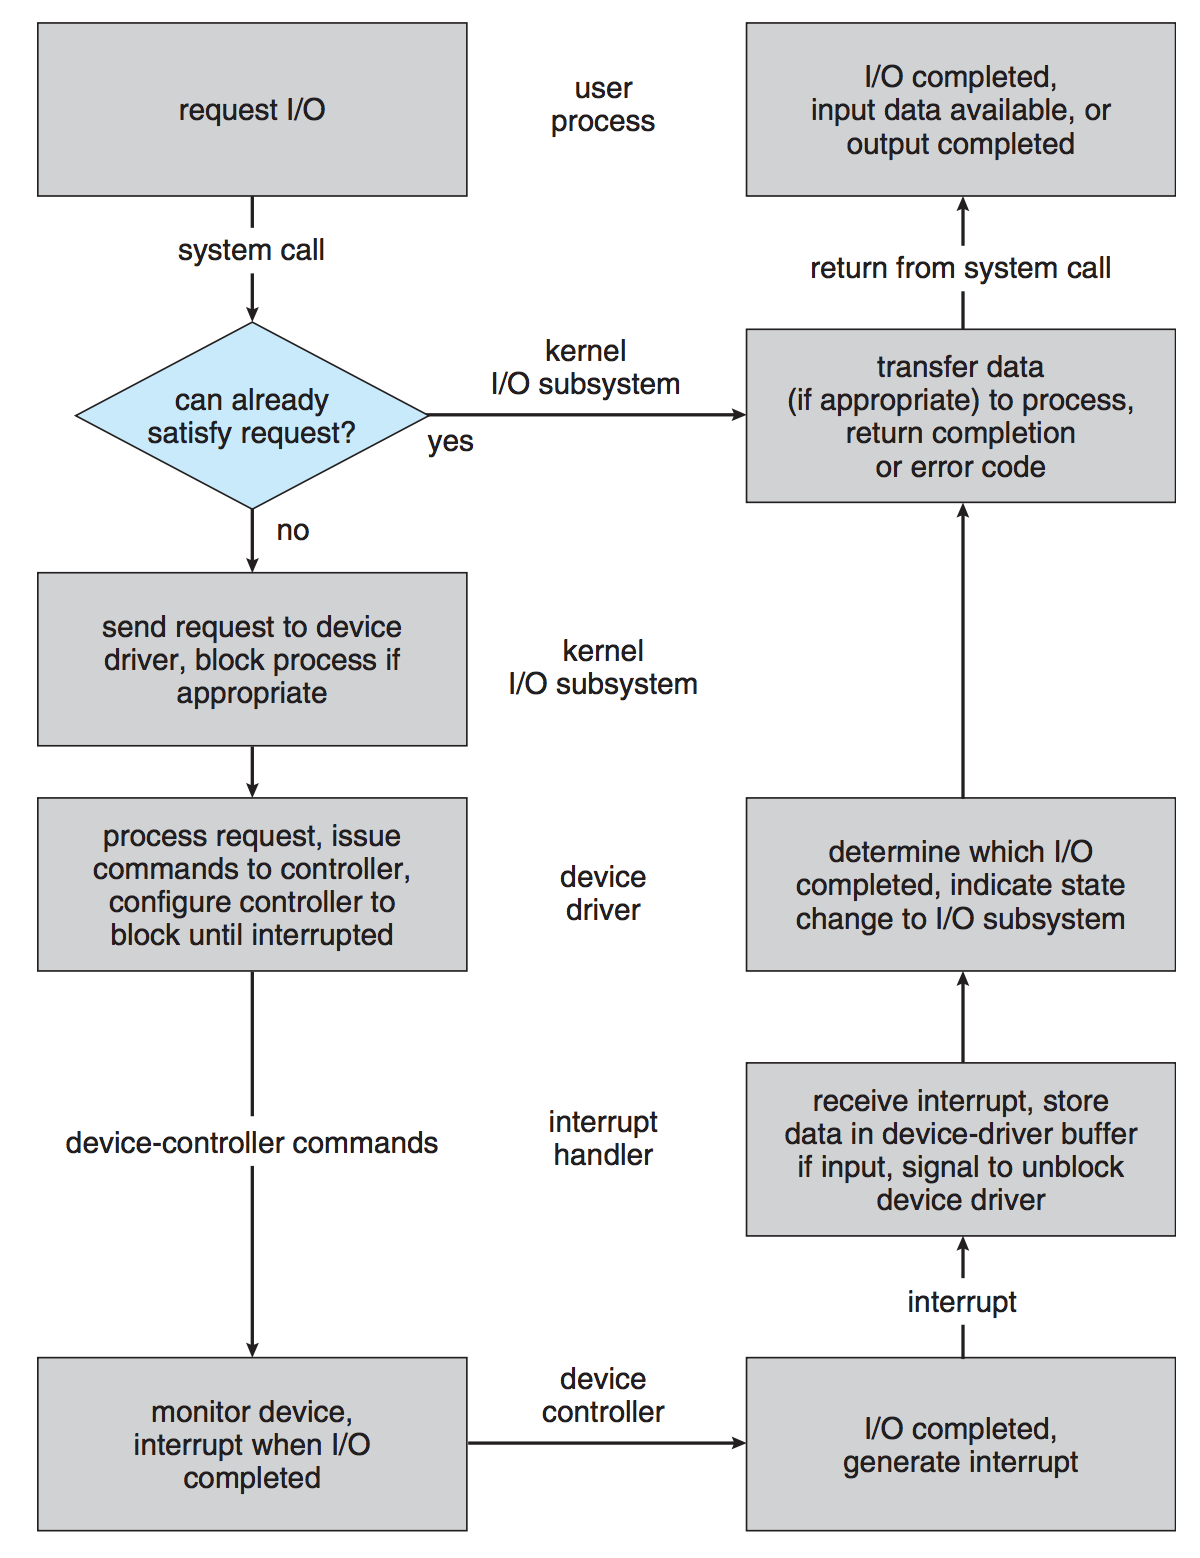
\includegraphics[width=0.5\textwidth]{images/io-lifecycle.png}
\end{center}

\end{frame}

\begin{frame}
\frametitle{Buffering}

Regardless of whether a device is block- or character-oriented, the operating system can improve its performance through the use of buffering. 

As you may have experienced, the use of a buffer speeds things up.

A buffer is nothing more than an area of memory that stores data being transferred, from memory to a device, device to memory, or device to device. 

\end{frame}


\begin{frame}
\frametitle{Buffering}

A buffer is a good way to deal with a speed mismatch between devices. 

Users type very slowly, from the perspective of the computer. 

It would be awfully inefficient to ask the disk, a block oriented device, to update itself on every single character. 

\end{frame}



\begin{frame}
\frametitle{Buffering, Please Wait}

Probably you're familiar with this from YouTube or similar:

\begin{center}
	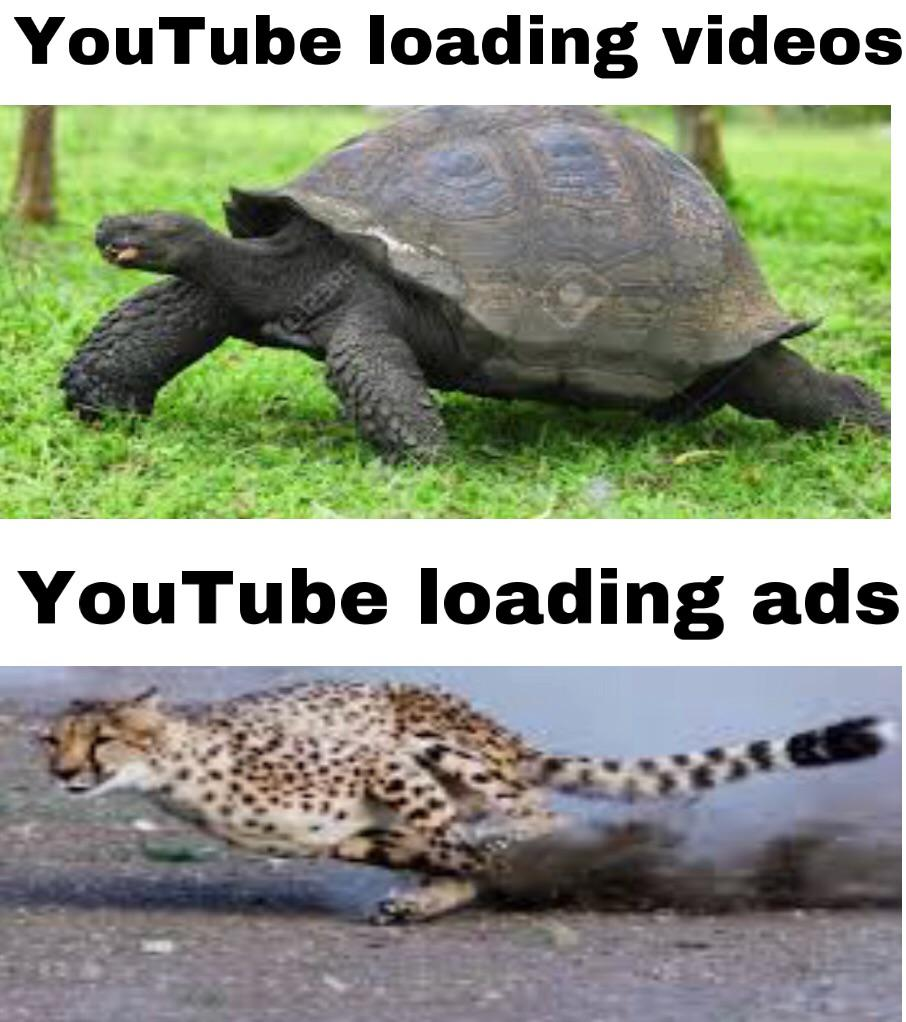
\includegraphics[width=0.4\textwidth]{images/buffering.jpg}
\end{center}

\end{frame}


\begin{frame}
\frametitle{Buffer Calculation}

We'll say $T$ is the time required to input one block and $C$ is the computation time between input requests. 

With no buffer, the execution time to complete a block is $T+C$.

With a buffer it is max$(C, T) + M$, where $M$ is the time to move the data from a system buffer to process memory.


\end{frame}



\begin{frame}
\frametitle{Capacity is Limited}

A buffer is normally created with a maximum capacity to it.

Sometimes we talk about unbounded buffers, but there's always a limit.


\end{frame}



\begin{frame}
\frametitle{Implementing a Buffer}

Implementing a buffer is relatively straightforward operation from the point of view of the operating system because it really only requires two operations. 

Add something to and remove something from the buffer.

Does that sound familiar?

\end{frame}


\begin{frame}[fragile]
\frametitle{Buffer Implementation}

\begin{multicols}{2}
	\textbf{Producer}
	\begin{verbatim}
	 1. [produce item]
	 2. wait( spaces )
	 3. wait( mutex )
	 4. [add item to buffer]
	 5. post( mutex )
	 6. post( items )
  \end{verbatim}
	\columnbreak
	\textbf{Consumer}
	\begin{verbatim}
	 1. wait( items )
	 2. wait( mutex )
	 3. [remove item from buffer]
	 4. post( mutex )
	 5. post( spaces )
	 6. [consume item]
  \end{verbatim}
\end{multicols}

Okay, how about now?

\end{frame}


\begin{frame}
\frametitle{Double Buffering}

Just a minute ago, we said typing should go into a buffer...

When the buffer is full, write it out to disk, right?

The write is not instantaneous and in the meantime, a user can still keep typing. 


\end{frame}


\begin{frame}
\frametitle{Double Buffering}


The typical solution is \alert{double buffering}, that is, two buffers. 

While buffer one is being emptied, buffer two receives any incoming keystrokes. 

Double buffering decouples the producer and consumer of data, helping to overcome speed differences between the two.

\end{frame}


\begin{frame}
\frametitle{Double Buffering}

The obvious extension is to have MORE buffers -- circular buffering.

\begin{center}
	
\includegraphics[width=0.4\textwidth]{images/flatcircle.jpg}
\end{center}

\end{frame}


\begin{frame}
\frametitle{Not Unlimited}

Buffering does not solve all problems...

Although it can smooth out peaks and valleys in producing and consuming, if one is consistently higher than the other, buffering doesn't help.


\end{frame}


\begin{frame}
\frametitle{I/O Scheduling and Performance}

The OS must keep track of in-progress I/O operations.

Like a semaphore, track the device status and have a queue for it.

How to manage the queue?

\end{frame}


\begin{frame}
\frametitle{History Rhymes}

When a thread wants to use the device, check the device status! 

If it's available then we can mark the device as busy and submit the request to the device. 

Until the operation is complete, mark the requesting thread as blocked. 

\end{frame}


\begin{frame}
\frametitle{History Rhymes}

If a thread shows up and wants to use a device that's already in use, just block it and add that thread to the queue. 

When the operation is complete, unblock the thread waiting for it and let it continue. 

If there are no further requests waiting, mark the device as idle (not in use). 

Otherwise, keep the status as busy and begin the next request.

\end{frame}


\begin{frame}
\frametitle{This is FCFS}

That's FCFS -- and maybe that's adequate.

It's fair, but perhaps not optimal.

Thought: what if devices have non-uniform access times?

\end{frame}

\begin{frame}
\frametitle{I/O Scheduling}

Sometimes we want to schedule I/O requests in some order other than First-Come, First-Served. 

Analogy: you need to go to the grocery store, the dry cleaners, and the bank. 

The bank is 1~km to the west of your current location; the grocery store is 3~km west; and dry cleaners is in the same plaza as the grocery store. 

It would be fine to go to the bank, then the dry cleaners, then the grocery store, but not to go to the dry cleaners, then the bank, then the grocery store. 

The unnecessary back-and-forth wastes time and energy.


\end{frame}

\begin{frame}
\frametitle{I/O Scheduling}
The operating system will want to do something similar with I/O requests.

Maintain requests structure; re-arrange them to be accomplished efficiently.

This will, naturally, have some limits: requests should presumably get scheduled before too much time has elapsed even if it would be ``inconvenient''. 

It might also take priority into account. 

\end{frame}


\begin{frame}
\frametitle{There Should be a Limit}

On the other hand, requests should get scheduled eventually.

There's tradeoffs between efficiency and fairness!


\end{frame}


\begin{frame}
\frametitle{Too Much of a Good Thing}

\begin{center}
	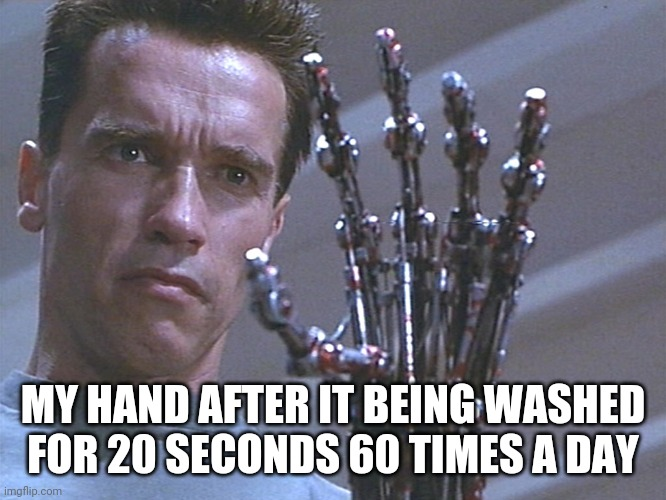
\includegraphics[width=0.4\textwidth]{images/terminator-hand.jpg}
\end{center}

We've discussed the idea already that interrupts are more efficient than polling, you might question if there's such a thing as too responsive. 

\end{frame}


\begin{frame}
\frametitle{Downloading a File Example}

For downloading a file, say, the number of interrupts is probably manageable.

As each chunk arrives, the interrupt is triggered, and the chunk is handled. 

Eventually, all the file is downloaded and there we are.

\end{frame}


\begin{frame}
\frametitle{Keyboard Interrupt}

Let's imagine I have \texttt{eceubuntu} open and I'm typing in an editor.

I press \texttt{Z} locally and then...
\begin{itemize}
	\item Keyboard interrupt locally
	\item Network request locally
	\item Network arrival remotely
	\item Editor processes keypress, updates screen
	\item Network request remotely
	\item Network arrival locally
\end{itemize}

\end{frame}


\begin{frame}
\frametitle{How to Reduce This?}

The book suggests some special hardware. 

\begin{center}
	
\includegraphics[width=0.4\textwidth]{images/crazypills.jpg}
\end{center}

But we \textit{have} looked at some specialized hardware: e.g., TLB.

Other ideas?
\end{frame}

\begin{frame}
\frametitle{Reducing Interrupt Overload}

Reduce the amount of time to handle an interrupt?

Wait for a bigger chunk of data?

Use DMA hardware?

\end{frame}


\begin{frame}
\frametitle{Security in I/O Devices}
Device drivers run at a high level of trust in the operating system, they offer an easy route for attackers!

\begin{center}
	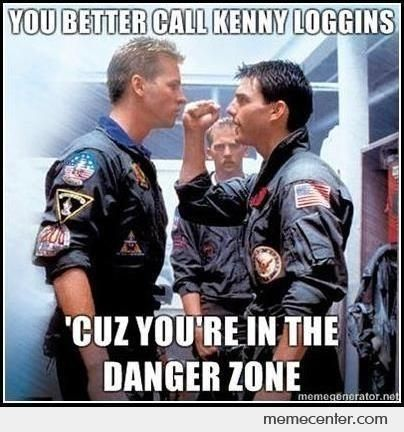
\includegraphics[width=0.4\textwidth]{images/dangerzone.jpg}
\end{center}

Attack vector: privilege escalation in a driver.

\end{frame}


\begin{frame}
\frametitle{But How?}

The vulnerable driver has to be on the target system in the first place. 

If an administrator wishes, they can intentionally install a driver with a known vulnerability to be able to do something bad. 

But admins can already do bad things?

\end{frame}


\begin{frame}
\frametitle{Bad Drivers}
Bad drivers should not get installed automatically because of driver signing that we talked about earlier on.

Trying to install a driver that's not signed tends to result in the operating system throwing a ton of warnings.

Do people ignore these?

\end{frame}


\begin{frame}
\frametitle{Found the Vulnerability Later?}
This doesn't solve the problem of what happens if there's a vulnerability in an otherwise-legitimate driver.

Such a driver would have been tested, approved, and signed and the problem is only discovered after the driver is released.

That doesn't prevent installing the old version with the vulnerability.

\end{frame}


\begin{frame}
\frametitle{Revocation}

What is needed is some idea of revocation: un-approve a driver.

Microsoft has not been properly applying updates to the driver block-list which resulted in exploitable drivers being installed.

\begin{center}
	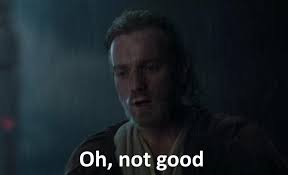
\includegraphics[width=0.4\textwidth]{images/notgood.jpg}
\end{center}

\end{frame}


\begin{frame}
\frametitle{That's a Bit Late}

Microsoft did address this once it was reported, but a little late. 

There were some known cases of actual exploits taking place using drivers in the block-list. 

And as you may imagine, the installation rate for patches to any operating system is never 100\%, so vulnerable systems will continue to exist...



\end{frame}



\end{document}

